\documentclass{beamer}
\mode<presentation>
\usepackage{amsmath}
\usepackage{amssymb}
%\usepackage{advdate}
\usepackage{adjustbox}
\usepackage{subcaption}
\usepackage{enumitem}
\usepackage{multicol}
\usepackage{listings}
\usepackage{url}
\usepackage{hyperref}
\hypersetup{
    colorlinks=true,
    linkcolor=blue,
    filecolor=magenta,      
    urlcolor=cyan,
}
\def\UrlBreaks{\do\/\do-}
\usetheme{Boadilla}
\usecolortheme{lily}
\setbeamertemplate{footline}
{
  \leavevmode%
  \hbox{%
  \begin{beamercolorbox}[wd=\paperwidth,ht=2.25ex,dp=1ex,right]{author in head/foot}%
    \insertframenumber{} / \inserttotalframenumber\hspace*{2ex}
  \end{beamercolorbox}}%
  \vskip0pt%
}
\setbeamertemplate{navigation symbols}{}


\numberwithin{equation}{section}

\title{EE2101 Control Systems\\Question 43}
\author{Srijith Reddy Pakala \\EE19BTECH11041\\ Dept. of Electrical Engg.,\\IIT Hyderabad.}

\date{\today}
\begin{document}

\begin{frame}
\titlepage
\end{frame}

\section*{Outline}
\begin{frame}
\tableofcontents
\end{frame}
\section{Problem}
\begin{frame}
\frametitle{Problem Statement}
The motor whose torque-speed characteristics are
shown in Figure 1 drives the load shown in the
diagram. Some of the gears have inertia. Find the
transfer function,G(s)=$\theta_2(s)/E_a(s)$.
\begin{center}
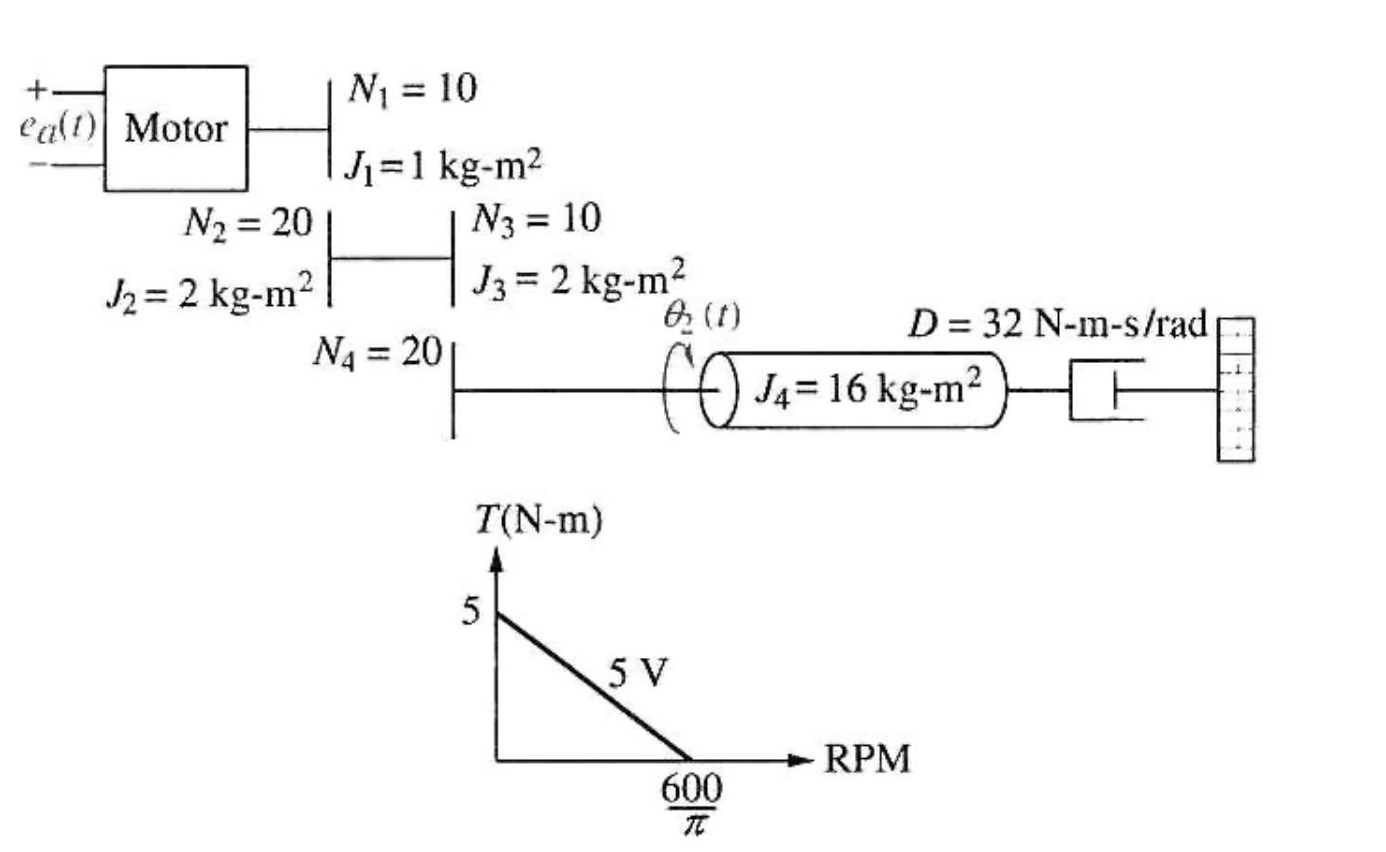
\includegraphics[width=0.8\columnwidth]{./figs/EE2101.png} \\
\end{center}
\begin{center}
\textbf{Figure 1} 
\end{center}
\end{frame}


\section{Solution}
\begin{frame}
\frametitle{Solution}
First we need to find the Mechanical constants $J_m$,$D_m$ in the equation(3.1)
\begin{equation}
 \frac{\theta_m(s)}{E_a}=\frac{K_t/R_aJ_m}{s[s+\frac{1}{J_m}(D_m+\frac{K_tK_b}{R_a})]}   
\end{equation} 
The total inertia at the armature of the motor is
\begin{equation}
J_m=J_1+(J_2+J_3)\bigg({\frac{N_1}{N_2}\bigg)}^2+J_4\bigg({\frac{N_1N_3}{N_2N_4}\bigg)}^2    
\end{equation}
The total damping at the armature of the motor is
\begin{equation}
D_m=D\bigg({\frac{N_1N_3}{N_2N_4}\bigg)}^2     
\end{equation}
\end{frame}
\begin{frame}{Solution}
Now we will find the electrical constants, $K_t$/$R_a$ and $K_b$.From the torque-
speed curve of Figure 2.\\
\begin{center}
  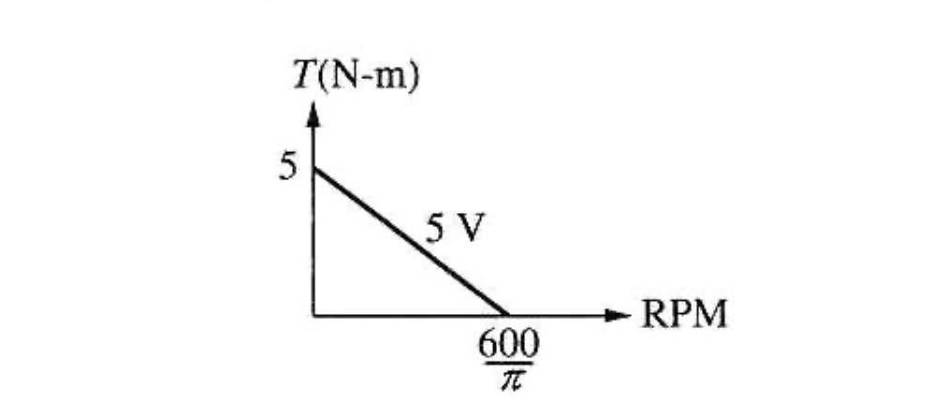
\includegraphics[width=0.5\columnwidth]{./figs/KK.png} \\
$T_{stall}$=5\\
$\omega_{no-load}=\frac{600}{\pi}$\\
$e_a$=5\\   
\end{center}


Hence the electrical constants are\\
\begin{center}
    $\frac{\big{K_t}}{\big{R_a}}$ = $\frac{\big{T_{stall}}}{\big{e_a}}$=$\frac{\big5}{\big5}$=1\\
\end{center}


\end{frame}
\begin{frame}{Solution}
and
\begin{center}
    $K_b$ = $\frac{\big{e_a}}{\big{\omega_{no-load}}}$=$\frac{\big5}{{\frac{\big{600}}{\big{\pi}}}\frac{\big{2\pi}}{\big{60}}}$=$\frac{\big1}{\big4}$\\
\end{center}
 The above equations are derived in the text book "Norman.Nise control systems engineering chapter 2.8"\\
 Given N_1=10,N_2=20,N_3=10,N_4=20\\
 and J_1= 1 kg-m^2,J_2= 2 kg-m^2,J_3= 2 kg-m^2\\
 ,J_4= 16 kg-m^2,
 and \space D= 32 N-m-s/rad\\
 \\

\end{frame}
\begin{frame}{Solution}
 By substituting above values in equations (3.2) , (3.3) we get \\
   J_m=1+(2+2)\bigg({\frac{\big1}{\big2}\bigg)}^2+16\bigg({\frac{\big1}{\big4}\bigg)}^2=3\\
   D_m=32\bigg({\frac{\big1}{\big4}\bigg)}^2= 2   \\
   Finally substituting all the variables in equation (3.1)\\
   \begin{center}
       $\frac{\big{\theta_m(s)}}{\big{E_a}}$=$\frac{\frac{\big1}{\big3}}{\big{s}\bigg[\big{s}+\frac{\big1}{\big3}\bigg(\big2+\frac{\big1}{\big4}\bigg)\bigg]}$ = $\frac{\big1}{\big{3s}\bigg[\big{s+0.75}\bigg]}$
   \end{center}
   
\end{frame}
\begin{frame}{Solution}

 Since   
 \begin{center}
 $\theta_2(s)$=$\frac{\big1}{\big4}\theta_m(s)$      
 \end{center}
  

Thus 
\begin{center}
\[
 \boxed{G(s)=\frac{\big{\theta_2(s)}}{\big{E_a}}$= $\frac{\big1}{\big{12s}\bigg[\big{s+0.75}\bigg]}}
 \]
    The code for the above calculations can be seen \href{https://github.com/SRIJITH01/EE2101/blob/master/EE19BTECH11041.py}{here}   
 \end{center} 
\end{frame}
\begin{frame}
   
\includegraphics[width=14cm, height=10cm]{./figs/thank.png} \\  
\end{frame}

\end{document}

